%%%%%%%%%%%%%%%%%%%%%%%%%%%%%%%%%%%%%%%%%%%%%%%%%%%%%%%%%%%%%%%%%%%
%                                                                 %
%  GEANT manual in LaTeX form                              %
%                                                                 %
%  Michel Goossens (for translation into LaTeX)                   %
%  Version 1.00                                                   %
%  Last Mod. Jan 24 1991  1300   MG + IB                          %
%                                                                 %
%%%%%%%%%%%%%%%%%%%%%%%%%%%%%%%%%%%%%%%%%%%%%%%%%%%%%%%%%%%%%%%%%%%
\Origin{R.Brun}
\Submitted{01.11.83}     \Revised{18.12.93}
\Version{Geant 3.16}     \Routid{HITS399}
\Makehead{The JDIGI data structure}

\begin{figure}[hbt]
     \centering
     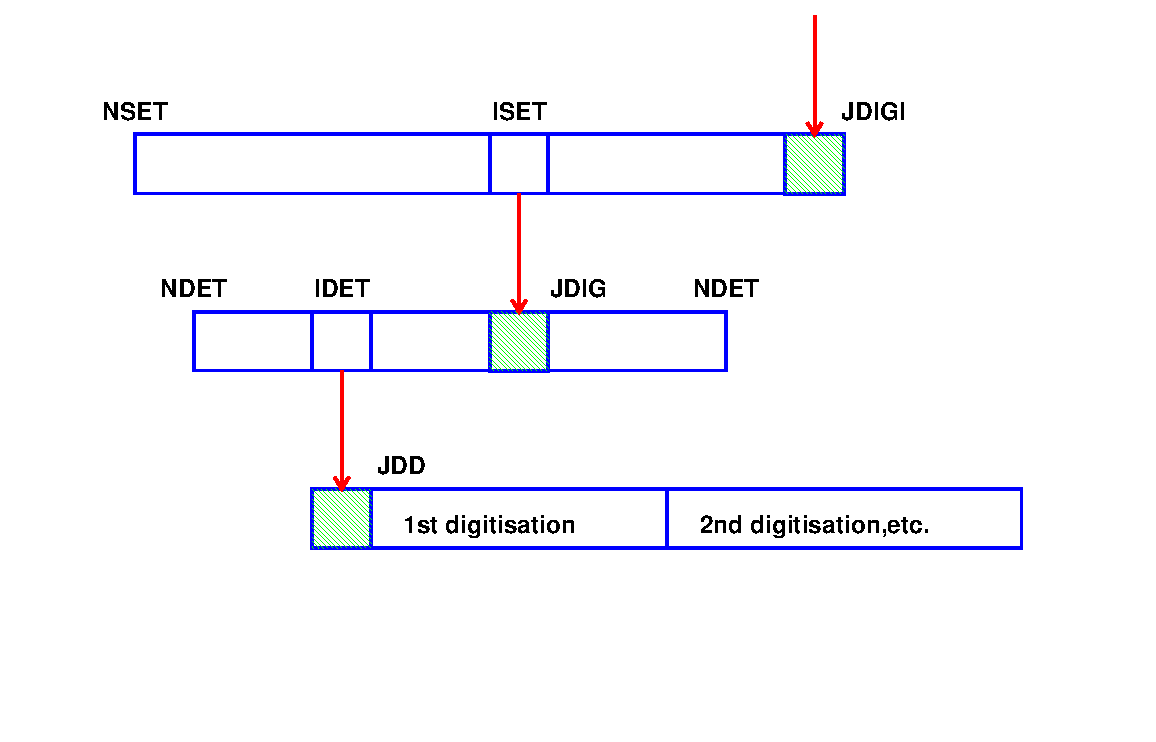
\epsfig{file=eps/hits399-1.eps,width=14cm}
     \caption{Layout of the {\tt JDIGI} data structure}
     \label{fg:hits399-1}
\end{figure}

\begin{tabular}{lp{10cm}}
\tt JDIG=LQ(JDIGI-ISET) & pointer to digitisations structure for set 
number {\tt ISET}\\
\tt JDD=LQ(JDIG-IDET) & pointer to digitisations of detector number
{\tt IDET} of set number {\tt ISET} \\
\tt IQ(JDIG+IDET) & pointer to last word of last digitisation for detector
number {\tt IDET} \\
\tt IQ(JDD+1) & 1$^{st}$ word of 1$^{st}$ digitisation \\
\tt IQ(JDD+N+1) & 1$^{st}$ word of 2$^{nd}$ digitisation\\
\tt JS=LQ(JSET-ISET) & pointer to the structure containing the description
of digitisations of set number {\tt ISET} \\
\tt JD=LQ(JS-IDET) & pointer to the structure containing the description
of digitisations of detector number {\tt IDET} \\
\tt NWD=IQ(JD+5) & number of elements of digitisation of set/detector
{\tt ISET}/{\tt IDET}  \\
\tt NTRA & number of tracks contributing to digitisation\\
\tt N=NWD+NTRA/2+1 & N varies from digitisation to digitisation 
\end{tabular}

The {\tt JDIGI} structure is filled with the routine \Rind{GSDIGI}.
The routine \Rind{GFDIGI} can be used to get the digitisations for
a detector {\tt IDET} in set {\tt ISET}.
 
